\section{Mindfulness meditation}
%Definition
Mindfulness is often defined as being in the mental state of Non-Elaborative, non-judgmental awareness \cite{Zeidan2012,Zeidan2016}. 
Practicing mindfulness meditation includes control over sensory, emotional and cognitive happenings. Hereby the ability to control these sensations without being distracted by them as so the ability to abstract from past and future representations of memory.
Two popular practices of mindfulness meditation, focused attention (FA) and open monitoring (OM) are of the most well practiced types of meditation. \cite{Zeidan2016}

\textbf{Focused attention}\\ 
FA is the training of concentration, where one keeps his or her focus at an object or specific thing, only focusing on that thing. Often the flow of breath is the focus, when practicing FA meditation.  When any disturbance comes by, like a thought, sound or other environmental distractions, which will often lead to a drift in attention, the person should always bring his or her attention back to the focus. \cite{Zeidan2016}

This kind of meditation has shown to enhance focus and concentration. ..

\textbf{Open monitoring}\\
OM is the cultivation of open presence, were the mind is open to anything, not focusing on any specific thing, just being in the present. If any thought or disturbance comes by, the thought or sensation should be noticed briefly, but then left without thinking more over it. It is believed that this form of meditation is easier to learn when the person masters the meditation of FA, whereby the OM form is easier to master. \cite{Zeidan2016}

This kind of meditation has been shown to reduce pain more compared to FA, likely because the areas of the brain affected during this form of meditation is...\cite{Perlman2010}

The neural mechanisms behind mindfulness meditation in reliving pain has been researched and in experiments where stimulating with nociceptive pain there has been shown an increase in activity of the orbitofrontal cortex when meditating. Participants telling that they are able to feel the pain but able to deal with it better during meditation focusing on the breath. 
The same mechanisms working in analgsia is not the same as the mechanisms during meditation, why the two methods don't interfere with each other. \cite{Jacob2016}

The different areas of the brain show either a reduction or increase in activity when performing meditation. When practicing meditation the person trains the mind, and areas of specific regions will grow. \cite{Zeidan2012} \fxnote{....need a bit more elaboration....}

\begin{figure}[H]
	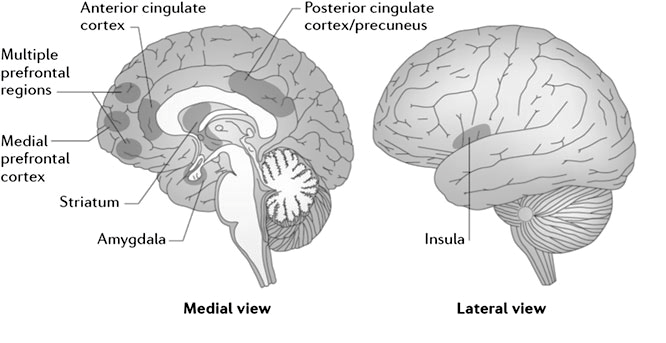
\includegraphics[width=0.8\textwidth,natwidth=610,natheight=642]{figures/brain_meditation.png} 
	\caption{Image of the brain and activation of specific brain regions when practicing meditation}
	\label{fig:brain_meditation}  
\end{figure}   
.... The figure needs to be changed to another one of better citation, but this was the best i could find by now :)....

The method of mindfulness meditation will not make the pain go away, but the patient will be able to deal with the pain easier, as mentioned, making the patient engage more in the treatment than focusing on and reeling on the medication. \cite{Jacob2016}
Very little mindfulness training can have an effect, the study by \cite{Zeidan2012} explaining an effect of training mindfulness meditation examined for 20 min sessions for 4 days of mindfulness meditation, but most studies conduct the experiments for a period of more than six weeks.  \cite{Zeidan2012}

FA and OM can alter pain in different ways...
OM is more effective in reducing pain after extensive meditation training compared to FA. 
\cite{Varilly2012}
                                      


